\documentclass{article}

\usepackage{hyperref}
\usepackage{listings}
\usepackage{color}
\usepackage[utf8]{inputenc} % usually not needed (loaded by default)
\usepackage[T1]{fontenc}
\usepackage{verbatimbox}
\usepackage{readarray}
\usepackage{amsmath,amssymb}
\usepackage{graphicx}
\usepackage{makeidx}
\usepackage{index}
\usepackage{hyperref}
\usepackage{array}
\hypersetup{
  colorlinks=true,
  linkcolor=blue,
  urlcolor=black,
  citecolor=black
}
\makeindex

% Margins
\topmargin=-0.45in
\evensidemargin=0in
\oddsidemargin=0in
\textwidth=6.5in
\textheight=9.0in
\headsep=0.25in

\title{ Introduction to Natural Language Processing, Assignment 1 }
\author{ Enrique Mesonero Ronco \and Sergio Sánchez García \and Ismael }
\date{\today}

\begin{document}
\maketitle
\begin{figure}[h!]
	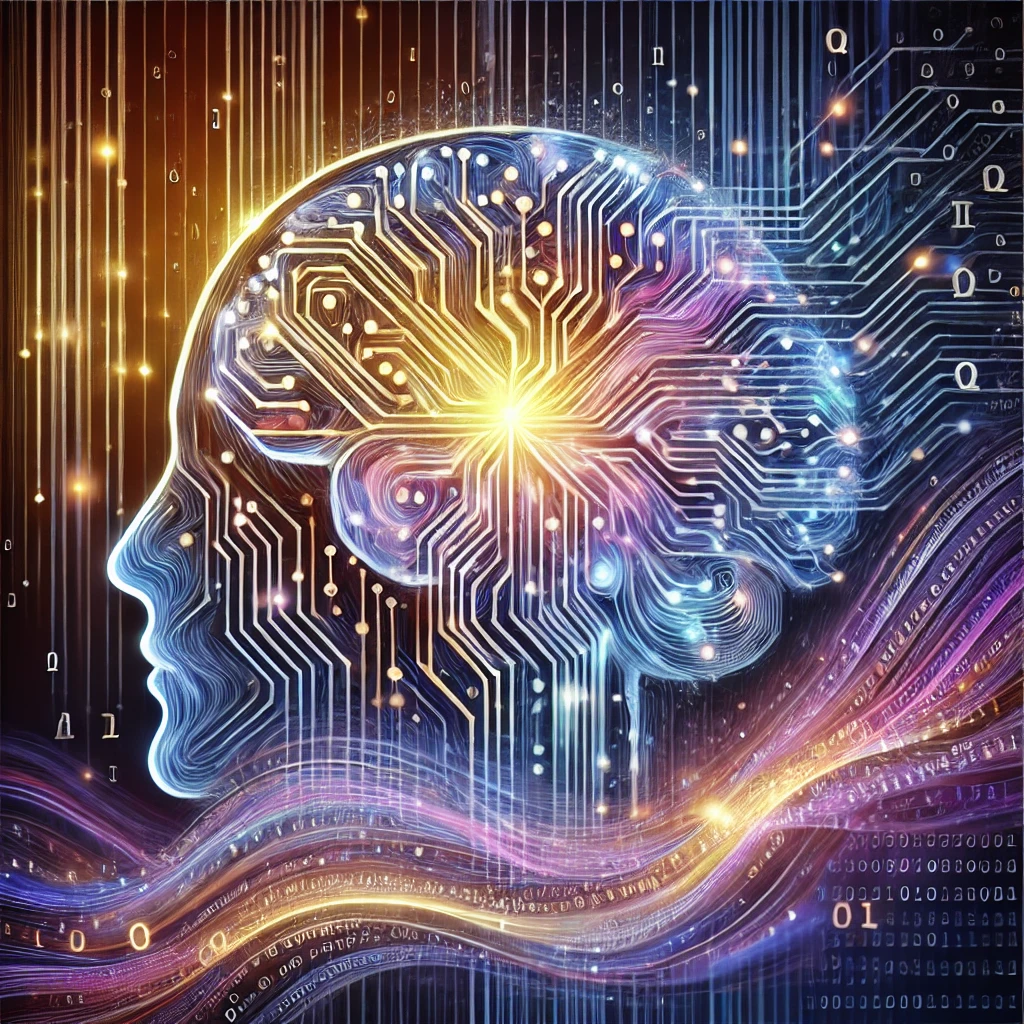
\includegraphics[width=\linewidth]{C:/Users/Enrique/Desktop/Clases/Introduction to NLP/Ejercicio 1/NLP.png}
\end{figure}
\newpage
\tableofcontents
\newpage
\section { Text Processing }
	\subsection { Tokenization }
	 \begin{itemize}
	\item First of all, it is necesary to lay down the initial base vocabulary:
		\begin{equation*}
			V_B = \{a,b,c,r,t\}
		\end{equation*}
		\begin{equation*}
			V_W (\text{as per} V_P) = \{b, a, t: 10; b, a, r: 5; c, a, t: 8; c, a, r: 4; c, a, r, t: 6\}
		\end{equation*}

	\item Secondly, merge tokens based on frequency:
		\begin{equation*}
			"c" + "a" \text{occur the most, 18 times in total}
		\end{equation*}
		\begin{equation*}
			V_B=\{a,b,c,r,t,ca\}
		\end{equation*}
		\begin{equation*}
			V_W={b, a, t: 10; b, a, r: 5; ca, t: 8, ca, r: 4; ca, r, t: 6}
		\end{equation*}
	\end{itemize}
	\subsection { Levenshtein Distance }

	\begin{center}
	\begin{tabular} { | m{1cm} | m{1cm} | m{1cm} | m{1cm} | m{1cm} | m{1cm} | }
		\hline
		 & \_ & H & U & N & D \\
		\hline
		\_ & 0 & 1 & 2 & 3 & 4 \\
		\hline
		H & 1 & 0 & 1 & 2 & 3 \\
		\hline
		A & 2 & 1 & 1 & 2 & 3 \\
		\hline
		N & 3 & 2 & 2 & 1 & 2 \\
		\hline
		D & 4 & 3 & 3 & 2 & 1 \\
		\hline
		Y & 5 & 4 & 4 & 3 & 2  \\
		\hline
	\end{tabular}
	\end{center}
hund $\rightarrow$ handy Total $\rightarrow$ 1 change operation + 1 add operation $\rightarrow$ Levensthein Distance = 2

	\begin{center}
	\begin{tabular} { | m{1cm} | m{1cm} | m{1cm} | m{1cm} | m{1cm} | m{1cm} | m{1cm} | }
		\hline
		 & \_ & N & A & T & T & Y \\
		\hline
		\_ & 0 & 1 & 2 & 3 & 4 & 5 \\
		\hline
		G & 1 & 1 & 2 & 3 & 4  & 5 \\
		\hline
		R & 2 & 2 & 2 & 3 & 4 & 5 \\
		\hline
		I & 3 & 3 & 3 & 3 & 4 & 5  \\
		\hline
		T & 4 & 4 & 4 & 3 & 3 & 4 \\
		\hline
		T & 5 & 5 & 5 & 4 & 3 & 4  \\
		\hline
		Y & 6 & 6 & 6 & 5 & 4 & 3  \\
		\hline
	\end{tabular}
	\end{center}
natty $\rightarrow$ gritty Total $\rightarrow$ 2 change operation + 1 add operation $\rightarrow$ Levensthein Distance = 3

\newpage
\section { Words and the Company They Keep }
	\subsection { Pearson's Chi-sqaure Test }
	\begin{center}
	\begin{tabular} { | m{2cm} | m{2cm} | m{2cm} | m{2cm} | }
		\hline
		 & B = $b_1$ & $B = b_2$ & Total \\
		\hline
		$A = a_1$ & 9 & 1770 & 1779  \\
		\hline
		$A = a_2$ & 75 & 219243 & 219318 \\
		\hline
		Total & 84 & 221013 & 221097 \\
		\hline
	\end{tabular}
	\end{center}

	\begin{equation*}
		 E_ij = \frac{f(w_i) \cdot f(w_j)}{N}
	\end{equation*}

\renewcommand{\arraystretch}{1.5}

	\begin{center}
	\begin{tabular} { | m{2cm} | m{2cm} | m{2cm} |  }
		\hline
		 & $B = b_1$ & $B = b_2$ \\
		\hline
		$A = a_1$ & $\frac{84 \cdot 1779}{221097}$ & $\frac{1779 \cdot 221013}{221097}$ \\
		\hline
		$A = a_2$ & $\frac{84 \cdot 219318}{221097}$ & $\frac{221013 \cdot 219318}{221097}$ \\
		\hline
	\end{tabular}
	\end{center}

\renewcommand{\arraystretch}{1}
	\begin{center}
	\begin{tabular} { | m{2cm} | m{2cm} | m{2cm} |  }
		\hline
		 & $B = b_1$ & $B = b_2$ \\
		\hline
		$A = a_1$ & 0.676 & 1778.32 \\
		\hline
		$A = a_2$ & 83.32 & 219234.6759 \\
		\hline
	\end{tabular}
	\end{center}
	\begin{equation*}
		\chi^2 = \sum_{i,j} \frac{(O_i,j - E_i,j)^2}{E_i,j}
	\end{equation*}
	\begin{equation*}
	\chi^2 = \frac{(9-0.676)^2}{0.676} + \frac{(1770-1778.32)^2}{1778.32} + \frac{(75-83.32)^2}{83.32} + \frac{(219243-219234.6759)^2}{219234.6759} = 102.5 + 0.04 + 0.83 + 3.16 \cdot 10^{-4} = 103.37
	\end{equation*}
	\subsection { PMI: Pointwise Mutual Information }

\end{document}